\usepackage{csquotes}\section{KI-basierende AMT-Systeme im Vergleich}
Im Laufe der Forschung zu AMT-Systemen wurden schon einige verschiedenen Architekturen eingesetzt und verbessert.
Jedes neue System hat, unabhängig des KI-Modells, eine komplett eigene Struktur und Vorgehensweise.
Im Verlauf dieser wissenschaftlichen Arbeit wurde die Geschichte von AMT-Systemen behandelt
und die wichtigsten Konzepte der automatischen Musiktranskription dargestellt.
Um dieses Forschungsgebiet zurück in die jetzige Gegenwart zu bringen,
handelt das letzte Kapitel von den heutigen \enquote{State of the Art} AMT-Systemen.
Dafür werden zwei verschiedene AMT-Systeme jetzt vorgestellt.
Diese sind das CNN + GRU basierte Omnizart und das Transformer-basierte MT3-Modell.
Diese nutzen unterschiedliche KI-Modelle.
Deren Architektur, sowie deren Stärken und schwächen, werden in dem folgenden Kapiteln ausgiebig erläutert.

\subsection{Omnizart}
Das erste System ist Omnizart, welches CNNs und GRUs als KI-Modelle nutzt \cite{wu2021omnizart}.
Der Name Omnizart setzt sich aus den Wörtern \enquote{Omni} (alles) und \enquote{Mozart} zusammen,
da ihr Ziel darin liegt, so viele Arten von Musik wie möglich zu transkribieren.
Je nach Anwendungsfall werden verschiedene KI-Systeme genutzt.
Dabei folgt der Aufbau dieser KI-Systeme meistens dem gleichen Schema.
Alle KI-Modelle bestehen aus einem CNN und einem bidirektionalen GRU.
Der Anwendungsfall, zum Beispiel Drums oder Melody, hat dabei nur Einfluss auf die Trainingsdaten und dem Output.
Omnizart ist ein Open-Source-Toolkit für AMT.
Dadurch lässt sich je nach Bedarf ein KI-Modell auswählen, das perfekt auf eine bestimmte Aufgabe ausgelegt wurde.
Omnizart findet seinen Ursprung im Jahre 2020 am Music and Culture Technology Lab, National Taiwan University.
Omnizart hat seit seiner Gründung keine ausschlaggebenden weiteren Technologien, in der Richtung KI, hinzugefügt.
Dafür gibt es für jeden vertretenen Anwendungsfall verschiedene CNNs und GRUs und einen open source code,
welcher gut zur eigenen Forschung an AMT-Systemen genutzt werden kann.
Omnizart ist ein modulares AMT-System, welches auf einer Deep-Learning-Architektur basiert.
Der Trainingssatz besteht aus CQT-Spektrogrammen.
Die KI-Modelle lernen dabei durch Supervised Learning.

Die Pipeline von Omnizart lässt sich in drei Schritte aufteilen:
\begin{figure}[H]
    \vspace{1em}
        \begin{tikzpicture}[>=stealth, thick]

            \node[align=right] at (-3,0) (label1) {\textbf{Preprocessing} \\ \footnotesize (Signalaufbereitung)};
            \node[align=right] at (-3,-2) (label2) {\textbf{KI-Modell} \\ \footnotesize (Merkmalerkennung)};
            \node[align=right] at (-3,-4) (label3) {\textbf{Postprocessing} \\ \footnotesize (Ausgabeaufbereitung)};

            \node at (1,0) (audio) {Audiodatei};
            \node at (5,0) (prep) {Preprocessing};
            \node at (9,0) (cqt) {CQT-Berechnung};
            \node at (1,-2) (cnn) {CNN};
            \node at (5,-2) (gru) {GRU};
            \node at (9,-2) (dense) {Dense-Layer};
            \node at (1,-4) (post) {Post-Processing};
            \node at (8.5,-4) (output) {MIDI/CSV/JSON/TXT}

            \draw[->] (audio) -- (prep);
            \draw[->] (prep) -- (cqt);
            \draw[->] (cqt.south) -- ++(0,-0.6) -| (cnn);
            \draw[->] (cnn) -- (gru);
            \draw[->] (gru) -- (dense);
            \draw[->] (dense.south) -- ++(0,-0.6) -| (post);
            \draw[->] (post) -- (output);

        \end{tikzpicture}
    \vspace{1em}
    \label{fig:omnizart}
    \caption[Omnizart Pipeline]{Eigene Darstellung der Omnizart Pipeline}
\end{figure}

Der erste Schritt ist die Vorverarbeitung und Merkmalsextraktion (Preprocessing).
Dadurch wird die Inputaudiodatei in ein CQT-Spektrogramm umgewandelt.
Zunächst wird das gegebene Audiosignal durch folgende Methoden standardisiert:
\begin{enumerate}
    \item \textbf{Mono-Konvertierung:} Die KI benötigt keine räumlichen Informationen, weshalb der linke und rechte Kanal von Stereosignalen in ein Monosignal addiert werden.
    \item \textbf{Normalisierung:} Der Wechsel von zu großen und kleinen Amplituden kann die KI überfordern und ungenaue Ergebnisse liefern, weshalb das Audiosignal durch Normalisierung auf einen einheitlichen Lautstärkebereich gebracht wird.
    \item \textbf{Resampling:} Unterschiedliche Abtastraten führen zu Verzerrung und Frequenzverschiebung, deshalb wird diese auf eine einheitliche Rate, passend zu dem genutzten Modul, gebracht.
    \item \textbf{Trimming:} Falls am Anfang oder Ende des Audiosignals Stille ist, wird diese durch Trimming entfernt, sodass das KI-Modell nicht unnötig verwirrt wird.
\end{enumerate}
Danach wird das standardisierte Audiosignal umgeformt zu einem CQT-Spektrogramm.

Im zweiten Schritt werden die KI-Modelle genutzt, um die Merkmale des Audiosignals vorherzusagen und zu extrahieren.
Die meisten AMT-Systeme, welche im Laufe dieser Arbeit vermerkt wurden, besitzen eine ähnliche Architektur wie Omnizart \cite{hawthorne2017onsets}.
Der Unterschied zu diesen AMT-Systemen ist das Omnizart, je nach Anwendungsfall, verschiedene Module nutzt.
Omnizarts Module sind:
\begin{itemize}
    \item \textbf{Chord:} Akkorderkennung
    \item \textbf{Drum:} Drum-Transkription
    \item \textbf{Melody:} Melodietranskription
    \item \textbf{Vocal:} Gesangsmelodietranskription
    \item \textbf{Piano:} Polyphone Klaviertranskription
    \item \textbf{Multi-Pitch:} Mehrstimmige Tonhöhenschätzung
    \item \textbf{Beat/Downbeat/Chord-Labelling:} Rhythmus, Takt \& Akkorde
\end{itemize}
Jedes Modul bekommt als Input ein CQT-Spektrogramm.
Dieses wird durch ein CNN verarbeitet, welches die Eigenschaften und Merkmale der Musik extrahiert.
Mit diesen Daten modelliert dann ein GRU die zeitliche Abhängigkeit.
Durch den Dense-Layer werden die Ergebnisse des GRUs in zum Beispiel Onsets,
Beats und zahlreiche weitere musikalischen Attribute, umgewandelt.

Im dritten Schritt wird der Output der KI-Modelle nochmals aufbereitet.
Fehler werden zunächst durch folgende Methoden verbessert:
\begin{enumerate}
    \item \textbf{Noten-Segmentierung:} Wenn derselbe Ton in zwei nacheinander folgenden Frame ein Onset hat, wird der zweite Onset gelöscht und der Note hinzugefügt, sodass keine Notendopplungen entstehen.
    \item \textbf{Onset-Korrektur:} Falls ein Onset zeitlich nicht zur richtigen Zeit erfasst wurde, wird der Einschwingzeitpunkt des Onset an seinen Frame genau angepasst.
    \item \textbf{Thresholding:} Noten, die nicht einen bestimmten Wahrscheinlichkeits-Threshold überschreiten, werden aussortiert.
    \item \textbf{Quantisierung:} Je nach Taktstruktur können Noten zeitlich angepasst werden, sodass diese besser in beispielsweise einen 3/4-Takt passen und das Stück somit rhythmischer ist.
\end{enumerate}
Je nach Modul, welches gerade genutzt wird, werden nur ein paar oder alle dieser Methoden eingesetzt.
Auch deren Parameter unterscheiden sich je nach Modul.
So hat das Drums-Modul ein viel kleineren Schwellwert als das Melodien-Modul bei Thresholding.
Danach werden die Vorhersagen in vollständige Noten (Onset, Sustain, etc.)
zusammengefasst und in das gewünschte Format übertragen.
MIDI ist dabei das wichtigste Format, da dieses die relevanten Daten der Transkription für verschiedene Musiksoftware besitzt.
Es gibt aber auch noch drei andere Formate die, je nach Modul, ausgegeben werden.
Fast immer wird auch eine CSV-Datei ausgegeben.
Darin befinden sich die Transkriptionsdaten, welche zur Analyse oder Forschung genutzt werden können.
JSON-Dateien werden in den Chord- und Beat-Modulen ausgegeben.
Dies liegt daran, dass JSON-Dateien verschachteltet Daten, wie Akkordfolgen über mehrere Takte, besser speichern können.
In ihnen werden vor allem Takt-Informationen und Daten für Akkorde gespeichert.
TXT-Dateien werden dahingegen nur wahlweise in Modulen genutzt.
Sie sind ausschließlich für Debugging dar, weshalb sie für die meisten Nutzer nicht relevant sind.
Die Daten werden, in einer TXT-Datei, in einer unstrukturierten Liste ausgegeben.

\subsection{MT3}
Das Transformer-Modell, welches jetzt näher erläutert wird, heißt MT3.
MT3 steht für \enquote{Multi-Task Multitrack Music Transcription}.
MT3 ist gleichzeitig der Name für das Transformer-basierte KI-Modell, als auch für das AMT-System, indem dieses KI-Modell veröffentlicht wurde \cite{gardner2021mt3}.
Diese beiden sind untrennbar voneinander, da sie zu einer End-to-End-Architektur gehören.
Das MT3-Modell bildet einen wichtigen Meilenstein für die Transformer-basierte automatische Musiktranskription.
MT3 ist das erste weit verbreitete Multi-Task-Transkriptionsmodell.
Das heißt verschiedene Transkriptionsaufgaben werden von einem einzigen Modell gelöst.
Frühere Modelle brauchten zum Beispiel für Drums und die Melody,
wie es bei Omnizart der Fall ist, verschiedene KI-Modelle.
Durch die Communityversion \enquote{YourMT3+} wird dieses KI-Modell immer weiter gepflegt und verbessert.

MT3 ist ein Transformer-Modell, welches spezifisch für Musiktranskription entwickelt wurde.
Es besteht grundlegend aus folgenden Bereichen:
\begin{figure}[H]
    \vspace{1em}
    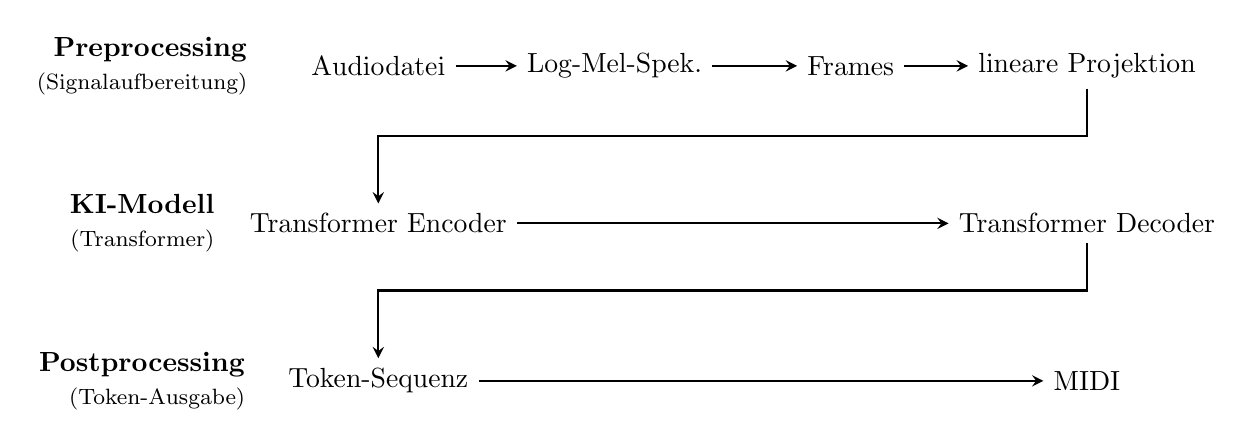
\begin{tikzpicture}[>=stealth, thick]

        \node[align=right] at (-3,0) (label1) {\textbf{Preprocessing} \\ \footnotesize (Signalaufbereitung)};
        \node[align=right] at (-3,-2) (label2) {\textbf{KI-Modell} \\ \footnotesize (Transformer)};
        \node[align=right] at (-3,-4) (label3) {\textbf{Postprocessing} \\ \footnotesize (Token-Ausgabe)};

        \node at (0,0) (audio) {Audiodatei};
        \node at (3,0) (logmel) {Log-Mel-Spek.};
        \node at (6,0) (frames) {Frames};
        \node at (9,0) (projection) {lineare Projektion};
        \node at (0,-2) (encoder) {Transformer Encoder};
        \node at (9,-2) (decoder) {Transformer Decoder};
        \node at (0,-4) (tokens) {Token-Sequenz};
        \node at (9,-4) (output) {MIDI};

        \draw[->] (audio) -- (logmel);
        \draw[->] (logmel) -- (frames);
        \draw[->] (frames) -- (projection);
        \draw[->] (projection.south) -- ++(0,-0.6) -| (encoder);
        \draw[->] (encoder) -- (decoder);
        \draw[->] (decoder.south) -- ++(0,-0.6) -| (tokens);
        \draw[->] (tokens) -- (output);

    \end{tikzpicture}
    \vspace{1em}

    \label{fig:mt3}
    \caption[MT3 Pipeline]{Eigene Darstellung der MT3 Pipeline}
\end{figure}

Als Input wird eine Audiodatei bereitgestellt.
Meistens wird der Datentyp WAV (Waveform Audio File Format) genutzt, da dieser verlustfrei und standardisiert ist.
Zudem wurde MT3 mit WAV-Dateien trainiert, weshalb es wenig Sinn macht einen anderen Datentyp zu nutzen.
Das Audiosignal wird dann mit STFT analysiert und als Spektrogramm ausgegeben.
Mithilfe von Librosa wird aus diesem ein Log-Mel-Spektrogramm erzeugt.
Librosa ist ein Python Paket, welches wichtige Methoden für Musik und Audio Analyse bereitstellt.
Dieses Log-Mel-Spektrogramm wird nun in Frames aufgeteilt.
In dem MT3-Modell sind diese Frames meist 32ms lang.
Jeder Frame besitzt N$x$Mel-Frequenzbänder, welche die Dimensionsgröße dieses Frames bestimmen.
Durch die Anzahl der Mel-Frequenzbänder wird die Frequenzauflösung des Inputs bestimmt.
In dem MT3-Modell werden standardmäßig 128 Mel-Frequenzbänder pro Fram genutzt.
Um jetzt für jeden Frame eine einheitliche Dimension zu bekommen,
mit der die KI arbeiten kann, wird lineare Projektion genutzt.
Lineare Projektion ist ein Matrix-Multiplikator, welche ein Frame auf eine,
für das KI-Modell, normalisierte Dimension bringt, zum Beispiel 512 oder 1024.
Daraus entstehen Input Embeddings, mit denen die KI jetzt arbeiten kann.

Jetzt folgt der Encoder, welcher das normale Prinzip eines Transformers,
mit Self-Attention Layer und Feedforward Layer, ausführt.
In dem MT3-Modell werden, vor der Ausführung der Layer,
die Positionen der Frames durch Positional Embeddings festgelegt.
In MT3 besteht der Encoder aus 6 vollständigen Transformer-Layern.
Der Inhalt jedes Frames wird jetzt mit dem aller anderen kontextabhängigen Frames zusammengeführt.
Daraus resultieren Vektoren, welche kontextreiche Informationen des Musikstückes besitzen.
Diese Vektoren werden weiter an den Decoder geleitet.

Aus den gegebenen Vektoren extrahiert der Decoder die wichtigen Daten.
Neben den Encoder Vektoren als Input bekommt dieser zudem autoregressive Tokens.
Autoregressive Tokens sind bereits generierte Tokens,
die im Training meist aus den echten Daten stammen (Teacher Forcing)
und beim Einsatz vom Modell, mithilfe der bereits generierten Tokens, selbst generiert werden.
Dadurch bekommt der Decoder mehr Kontext für die zu generierenden Tokens.
Neben den normalen Tokens bekommen auch die autoregressiven Tokens Positional Embeddings.
Bevor der Decoder nun durchläuft, lässt sich mithilfe von Task-Conditioning ein Task-Token hinzufügen.
Das MT3-Modell transkribiert immer polyphon, jedoch kann durch den Task-Token trotzdem der Output auf
einen bestimmten Task, wie zum Beispiel Klavierstücke oder Trommelnoten, ausgelegt werden.
Durch vorheriges Lernen ist das MT3-Modell darauf ausgelegt,
nach einem Task-Token die folgenden Tokens in einer bestimmten Art und Weise zu transkribieren.
Der Ablauf des Decoders sieht folgendermaßen aus:
\begin{enumerate}
  \item \textbf{Self-Attention:} verarbeitet den Kontext der autoregressiven Tokens
  \item \textbf{Cross-Attention:} extrahiert relevante Informationen aus dem Encoder-Output
  \item \textbf{Feedforward Layer:} verfeinert die Repräsentationen der Tokens lokal
  \item \textbf{Lineare Layer:} wandelt den Vektor in ein konkretes Token um
\end{enumerate}
Dabei besteht der Decoder, im MT3-Modell, auch aus 6 vollständigen Transformer-Layern.
Jeder Token stellt einen Teil eines musikalischen Events dar.
Diese heißen zum Beispiel \enquote{Note-On C4} oder \enquote{Shift +10 ms}.
Ein \enquote{Shift} von beispielsweise 10ms bedeutet, dass das nächste Ereignis 10 Millisekunden nach vorne in der Zeitleiste verschoben wird.
Ein musikalisches Event ist eine volle Note, mit Notennamen, Onset und Offset,
Sustain und weiteren musikalischen Eigenschaften, die auf einer Note angewendet werden können.
Als Output gibt der Decoder jeden einzelnen Token zurück.

Jetzt werden im Post-Processing die Tokens zu Sequenzen (musikalischen Events) zusammengesetzt.
Durch einige weitere Tools werden die Noten zudem noch bereinigt und verbessert.
\begin{itemize}
  \item \textbf{Zeitberechnung:} Die Shift-Tokens werden aufsummiert, sodass alle Noten zur richtigen Zeit abgespielt werden.
  \item \textbf{Noten validierung:} Jede Note wird darauf geprüft, ob sie ein On- und Offset besitzt.
  \item \textbf{Velocity Korrektur:} Manche Noten haben keine oder eine fehlerhafte Anschlagstärke, welche bei diesem Schritt im Nachhinein hinzugefügt oder überschrieben wird.
  \item \textbf{Fehlerbereinigung:} Unlogische Notenfolgen, wie zwei Shifts hintereinander, werden entfernt.
\end{itemize}
Am Ende werden die bereinigten Noten in einem standardisierten Musikformat, als MIDI-Datei, ausgegeben.

In der folgenden Darstellung ist der Transkriptionsablauf des MT3-Modells dargestellt.
Für den Input wird ein Audiosignal angegeben, welches in ein Spektrogramm umgewandelt wird.
Als nächstes gewichtet der Encoder, mithilfe der Self-Attention Layer, die Tokens und transformiert dann diese,
mithilfe des Feedforward Layer, um nicht-lineare Merkmale pro Token zu extrahieren.
Daraufhin wandelt der Decoder, die vom Encoder gegebenen Vektoren, in einzelne Tokens mit musikalischen Merkmalen um.
Im Output ist oben ein Ausschnitt einer MIDI-Datei mit zwei Noten zu sehen und darunter diese dargestellt als Piano-Roll.
\begin{figure}[H]
    \centering
    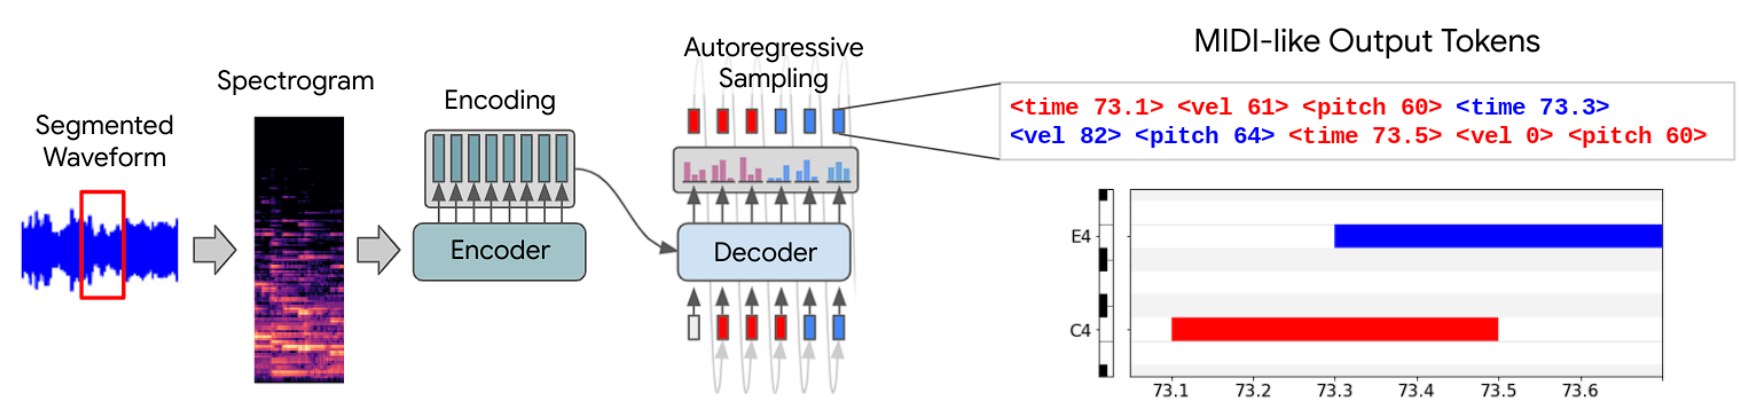
\includegraphics[width=1\textwidth]{Graphics/transcription_transformer}
    \caption[Verarbeitungspipeline des MT3-Modells]{Verarbeitungspipeline des Transformer-basierenden MT3-Modells  \cite{mt3colab}.}
    \label{fig:mt3_process}
\end{figure}

\subsection{Bewertung der AMT-Systeme im Vergleich}
Die beiden vorgestellten AMT-Systeme sind grundlegend verschieden aufgebaut.
Jetzt ist die Frage, welches dieser beiden Systeme besser geeignet ist.
Bei welchem Anwendungsfall und unter welchen Voraussetzungen sollte man welches System wählen?

Der größte Unterschied in der Architektur liegt darin,
das Omnizart verschiedenen KI-Modelle für unterschiedliche Aufgaben besitzt,
während MT3 ein einziges leistungsstarkes KI-Modell besitzt.
Somit lässt sich bei Omnizart leichter ein bestimmter Task verbessern oder analysieren.
Das ist vor allem gut, wenn der Fokus auf monophonen Musikstücken liegt
und ein einfacherer Einstieg in die automatische Musiktranskription erreicht werden soll.
Zudem gibt Omnizart eine größere Menge an Outputdaten zurück als MT3, bei dem nur eine MIDI-Datei ausgegeben wird.
MT3 hingegen besitzt ein einziges KI-Modell, wodurch kein spezieller Task gezielt umstrukturiert werden kann.
Dafür eignet sich das KI-Modell direkt das Wissen der verschiedenen Tasks an und kombiniert diese.
Somit können polyphone Musikstücke deutlich besser transkribiert werden.
Durch YourMT3+ gibt es zudem weiteres Ausbaupotential.
Dahingegen entwickelt sich Omnizart nicht sonderlich weiter.

Bei den KI-Modellen hat MT3 einen klaren Vorsprung.
CNNs und GRUs sind schon seit längerem in AMT-Systemen vertreten.
Sie wurden ausgiebig angepasst und verbessert für diesen Anwendungsfall.
Hingegen zu diesen KI-Modellen ist das MT3 erst seit paar Jahren im Rennen.
Durch YourMT3+ wird es immer weiter entwickelt,
wodurch es in der nahen Zukunft zu einem Standard der automatischen Musiktranskription werden könnte.
Zudem ist das MT3-Modell deutlich besser auf polyphone Musikstücke ausgelegt.
In der Mehrheit von Audiosignalen gibt es mehrere Stimmen.
Die meisten Menschen möchten auch lieber eine einfache Lösung, die wenig Eigenaufwand benötigt.
Deshalb wäre ein zentrales KI-Modell, zur Transkribierung von allen verschiedenen Audiosignalen, die populärste Lösung.
Ein Schwachpunkt des MT3-Modells ist der Rechenaufwand.
Alle KI Prozesse werden durch ein KI-Modell gelöst.
Deshalb muss dieses umso mehr Rechenschritte durchführen und braucht exponentiell mehr GPU Auslastung und Speicherkapazität.

Omnizart ist empfehlenswert, falls gerade ein neuer Einstieg in das Forschungsgebiet erfolgt.
Fortschritte werden deutlich schneller sichtbar, und der Fokus kann zunächst auf kleinere KI-Modelle gelegt werden.
In den meisten anderen Fällen wäre jedoch das MT3-Modell oder das Nachfolgermodell YourMT3+ empfehlenswerter.
Dieses ist der \enquote{State of the Art} und wird auch noch in einigen Jahren Support erhalten.
Zudem bestehen bei diesem Modell keinerlei Einschränkungen, und jegliche Musik kann transkribiert werden.
Dieses Modell geht jedoch auch mit viel Rechenaufwand und einem guten Verständnis des Forschungsgebiets einher.
Deshalb sollte vor der Nutzung des MT3-Modells eine gründliche Auseinandersetzung damit erfolgen.